%!TEX root = ../../../super_main.tex
\section{Implementation of New Design}
\label{sec:implementation_of_new_design}

The implementation of the design from \secref{sec:improved_design} has has been partially implemented during the second sprint. The main goal of second sprint in regards to the \ct was to implement the institute level, where guardians were able to create categories for an entire institution that could later be copied to citizens.\\

As mentioned previously the user is greeted by a homescreen where they can see their current categories or add new ones. This can be seen in \figref{fig:ct_home_screen}

\begin{figure}[!htbp]
    \centering
    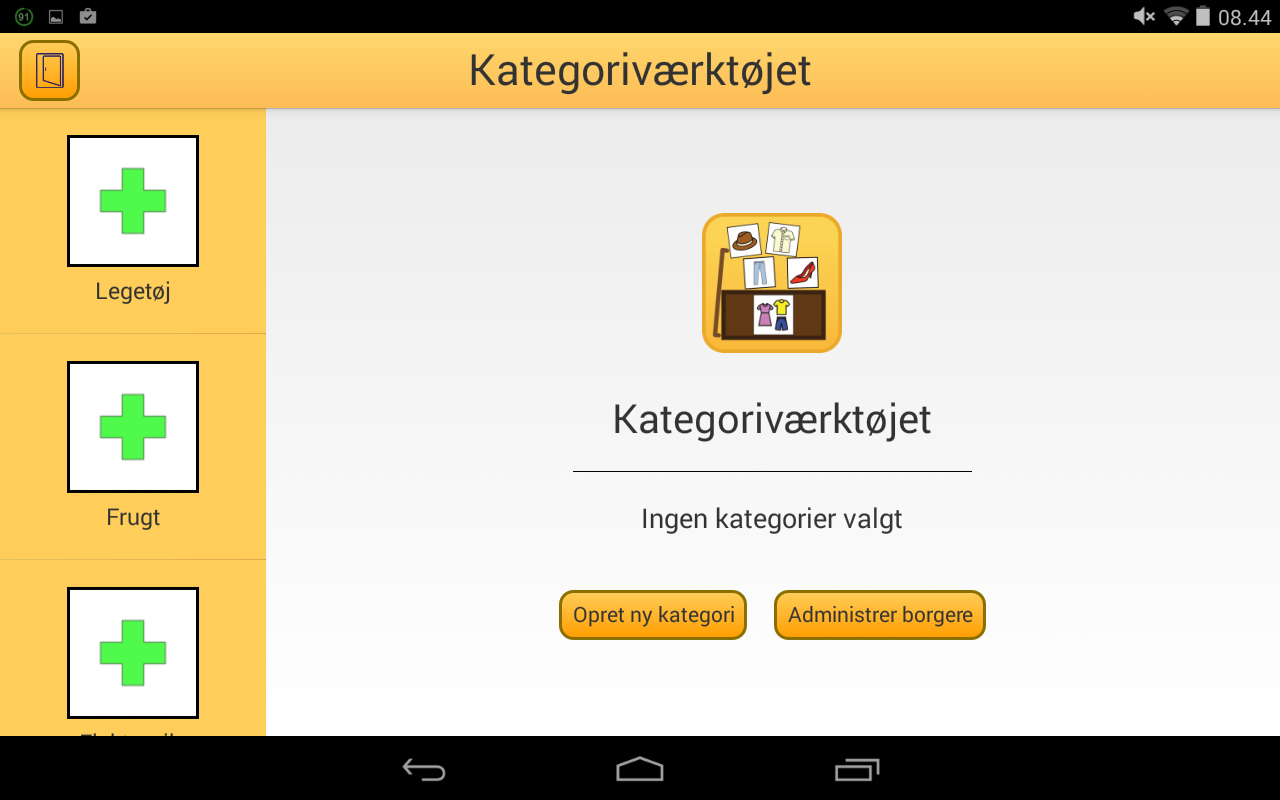
\includegraphics[width=\textwidth]{sprint_two/implementation_of_new_design/homescreen}
    \caption{\ct home screen}
    \label{fig:ct_home_screen}
\end{figure}

If the user selects a category, the pictogram list for that category will be shown, which can be seen in \figref{fig:ct_category_view}.\\

\begin{figure}[!htbp]
    \centering
    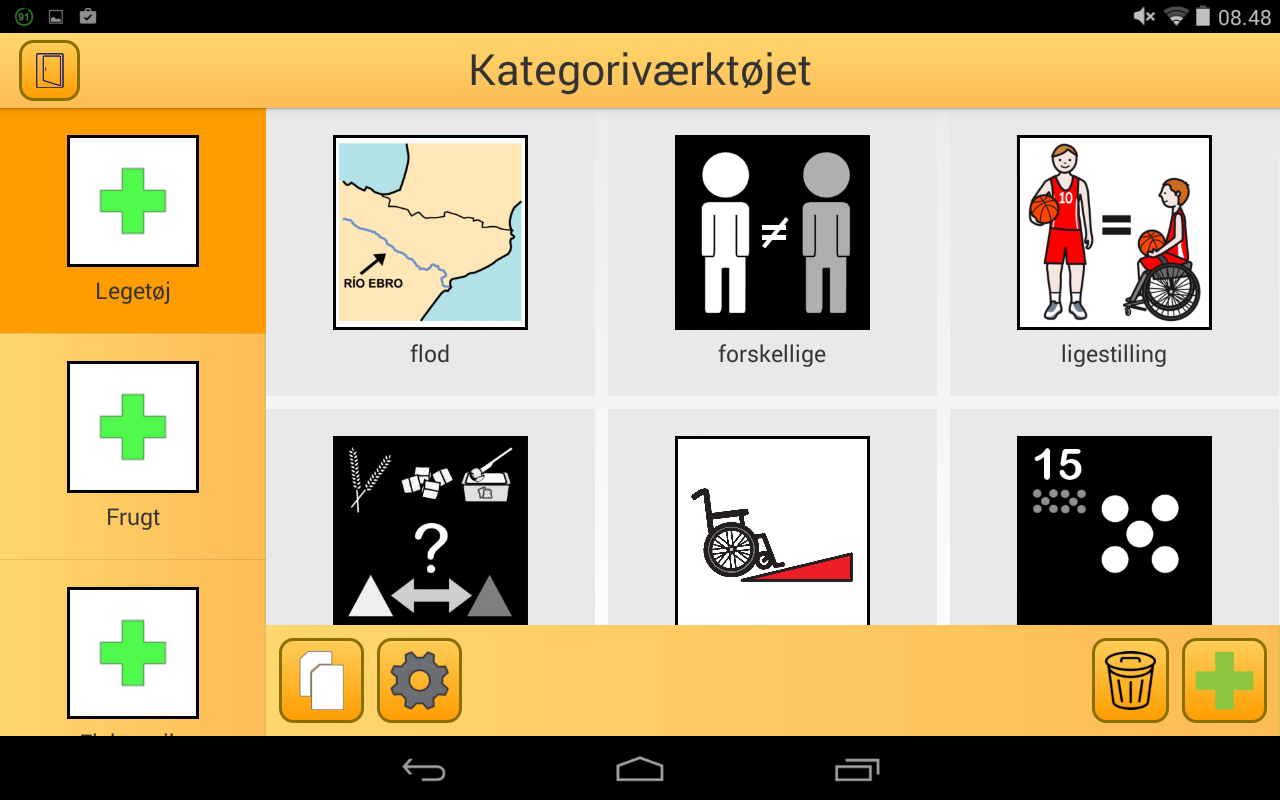
\includegraphics[width=\textwidth]{sprint_two/implementation_of_new_design/categoryview}
    \caption{\ct category view}
    \label{fig:ct_category_view}
\end{figure}


Both the list of categories as well as the list containing pictograms related to the category have been implemented using ListViews and Adapters, which makes sure that items in the list are only loaded when the users scrolls past it. This makes sure that excessive amounts of memory will not be used to store the complete list of queried categories or pictograms, and thereby make sure that the application does not crash because of lack of memory. 

The functionality of selecting a pictogram in a category has furthermore been implemented, but the visual cue that tells the user which pictogram is selected has not currently been implemented. We do however plan to continue with the \ct next sprint. 